\chapter{Modell} \label{Modell}
In diesem Kapitel erstelle ich ein Modell für den Fahrgastwechsel, und erkläre wie durch dieses die Ergebnisse der Datenauswertung umgesetzt werden. Zunächst beschreibe ich jedoch das bisher verwendete Modell von accu:rate. Daraufhin erstelle ich das Fahrgastwechsel-Modell. Dabei beschreibe ich auch das kognitive Heuristik Modell, auf dem mein Fahrgastwechsel-Modell aufbaut. Nachdem ich das Modell, die Umsetzung der Auswertung und die Grenzen des Modells erklärt habe, beschreibe ich dann den Algorithmus für dieses und die benötigten Parameter.
\section{Modell von accu:rate} \label{Accurate Modell}
Schon in früheren Projekten hat, accu:rate, Personenströme an U-Bahnstationen in München simuliert. Bis jetzt warten, in der Modellierung von accu:rate, die Personen rechts und links der Türen in Wartezonen. Diese Modellierung wird dabei vom Nutzer ertellt und ist nicht in der crowd:it Software implementiert. Die Wartezeit wird bei diesem Modell vor der Simulation festgelegt. Die Wartezeit wird bestimmt, indem berechnet wird wie lange die sich im Zug befindeten Personen, benötigen, um auszusteigen. Nach Ablauf der Wartezeit beginnen die wartenden Personen den Zug zu betreten. Da, wie in \ref{Stand der Technik} erwähnt, das Modell von accu:rate jedoch nicht auf empirischen Beobachtungen beruht, erstelle ich im Nachfolgenden ein Fahrgastwechsel-Modell, das ich auf Grundlage der angestellten Auswertungen der Daten erstellt habe. Das Modell erweitert crowd:it um kognitive Entscheidungsprozesse, sodass zukünftig nicht dem Nutzer das Modellieren von Verhalten überlassen werden muss, sondern die Software selbst das Verhalten abbilden kann. Diese Entscheidungsprozesse verwenden dabei Heuristiken des kognitiven Heuristik Modells nach \cite{Seitz.2016}. 
\section{Fahrgastwechsel-Modell} \label{Fahrgastwechsel-Modell}
Das Fahrgastwechsel-Modell modelliert den Ein- und Ausstiegsprozess sowie den Platzmachprozess. Für diese Prozesse werden unterschiedliche Heuristiken verwendet. In jeder dieser Heuristiken gibt es zudem Unterschiede für die unterschiedlichen Typen: aggressiv, defensiv und normal. \\
Das Fahrgastwechsel-Modell habe ich mit Hilfe des kognitiven Heuristik Modell umgesetzt, welches von Michael Seitz in seiner Dissertation vorgestellt wird (\cite{Seitz.2016}). Dieses Modell ist in der Software crowd:it zwar implementiert worden, wurde jedoch noch nicht für alle Fälle empirisch untersucht und getestet. Deshalb wird dieser Teil im Moment nicht verwendet. In der Dissertation von Michael Seitz überprüft dieser jedoch sein Modell mit zwei Szenarien durch Simulationen. Mit den Ergebnissen dieser Simulationen wird sein Modell durch den Vergleich mit den Ergebnissen aus kontrollierten Experimenten validiert. Dabei wurden zum einen die Ergebnisse für das Gehen durch einen Engpass (eng.: "`bottleneck"'), zum anderen die Ergebnisse eines bidirektionalen Flusses durch einen Korridor verglichen (\cite{Seitz.2016}). Mit eben diesen Szenarien kann der Fahrgastwechsel beschrieben werden. Wenn die Personen beim Fahrgastwechsel gleichzeitig ein- und aussteigen, kann dies als bidirektionaler Fluss durch einen Korridor beschrieben werden. Steigen Personen nur ein oder aus, so bewegen sich die Personen durch die Tür die als Engpass gesehen werden kann. In seiner Arbeit kommt \cite{Seitz.2016} zu dem Ergebnis, dass sein Ansatz für eine Fußgängersimulation mit diesen Szenarien geeignet ist. Nachdem genau die Szenarien untersucht wurden, mit denen ein Fahrgastwechsel beschrieben werden kann, nehme ich an, dass ich das Fahrgastwechsel-Modell auf diesem aufbauen kann. Das kognitive Heuristik Modell nach \cite{Seitz.2016} erkläre ich in Abschnitt \ref{CHM}.

Im dem von mir erstellten Fahrgastwechsel-Modell modelliere ich das Verhalten der Personen auf dem Bahnsteig und im Zug nicht, sondern nur der Fahrgastwechsel an sich. Soll in Zukunft auch das Verhalten im Inneren des Zuges und am Bahnsteig simuliert werden, kann mein Modell mit anderen bereits existierenden kombiniert werden. Für das Verhalten Einsteiger und Platzmacher nach dem Einsteigen kann das Modell der Sitzplatzwahl verwendet werden, dass Jakob Schöttl in seiner Masterarbeit an der Hochschule München erstellt hat (\cite{Schottl.2016}). Nachdem Aussteiger den Zug verlassen haben, kann zudem das bereits von crowd:it verwendete "`Optimal Steps"'-Modell für den weiteren Pfad der Aussteiger verwendet werden.
\subsection{Das kognitive Heuristik Modell} \label{CHM}
\cite{Seitz.2016} stellt in seiner Dissertation vier Heuristiken vor: die "`Step or wait"'-Heuristik, die "`Tangential evasion"'-Heuristik, die "`Sideways evasion"'-Heuristik und die "`Follower"'-Heuristik. Ich verwende die englischen Bezeichnungen im Folgenden weiterhin, um Verwirrungen durch undeutliche Übersetzungen zu verhindern. Bei der "`Step or wait"'-Heuristik gehen Personen einen Schritt in die Richtung des Ziels, wenn ihr Pfad frei ist und verbleiben in ihrer derzeitigen Position, falls nicht. Die "`Tangential evasion"'-Heuristik bringt Personen dazu, tangential auszuweichen, wenn ihr Pfad blockiert wird. Die "`Sideways evasion"'-Heuristik bringt Agenten zusätzlich dazu, seitlich auszuweichen, falls die "`tangential evasion"' nicht möglich ist. Die "`Follower"'-Heuristik lässt Agenten einen anderen Agenten suchen dem gefolgt werden kann, der in die gleiche Richtung geht, wenn der direkte Pfad zum Ziel blockiert wird (\cite{Seitz.2016}). Die Algorithmen für diese Heuristiken werden in \ref{Algorithmus} beschrieben. \\
Bei der Simulation mit der kognitiven Heuristik wird den Agenten zu Beginn ein Ziel zugeordnet. Wenn sie ihr Ziel erreicht haben, gehen sie entweder zu ihrem nächsten Ziel oder werden aus dem Szenario entfernt, wenn dieses Ziel ihr finales Ziel ist (\cite{Seitz.2016}). Für den Fahrgastwechsel bedeutet das, dass für Aussteiger die Ziele auf dem Bahnsteig hinter dem Wartebereich der Einsteiger liegen.
Die Skizze mit eingezeichnetem Ziel-Bereich für Aussteiger kann in \figurename \ref{fig:SkizzeAussteiger} betrachtet werden. Der Zielbereich der Aussteiger ist in dieser Abbildung durch rote Rechtecke gekennzeichnet.
\begin{figure}[H]
	\centering
		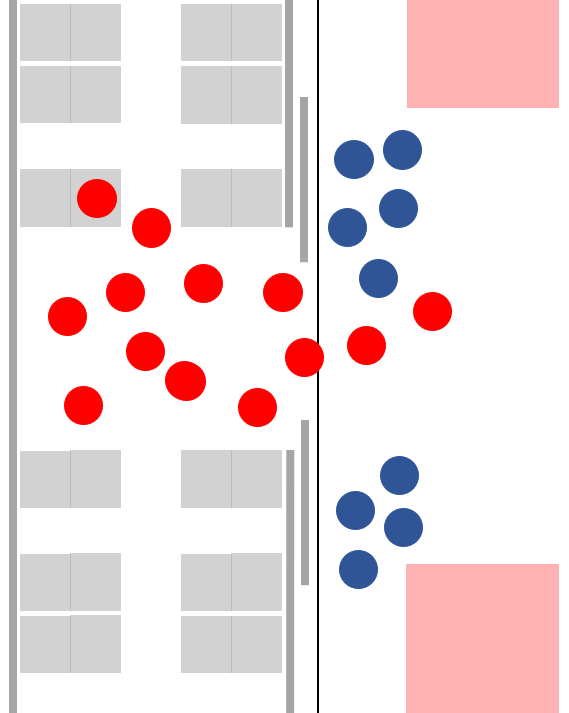
\includegraphics[angle=270, width=0.5\textwidth]{pictures/model/kognitive_heuristic_model/alight_sketch.png}
	\caption{Skizze zur Darstellung der Zielbereiche von Aussteigern aus der Vogelperspektive: U-Bahn "`Wände"' dargestellt durch graue Linien, Sitzplätze der U-Bahn durch graue Vierecke, Bahnsteigkante durch schwarze Linie, Aussteiger durch rote Kreise und Einsteiger durch blaue Kreise. Der Zielbereich ist mit einem roten Rechteck gekennzeichnet.}
	\label{fig:SkizzeAussteiger}
\end{figure}
Einsteiger und Platzmacher besitzen als Zwischenziel den Wartebereich. Einsteiger beginnen den Fahrgastwechsel am Bahnsteig in einigem Abstand vom Gleis. Von diesem Startpunkt bewegen sie sich zum Zwischenziel, einen Wartebereich rechts oder links der Türen. Ihr endgültiges Ziel liegt im Wagon kurz hinter den Türen.
Die Skizze für die Bereiche der Einsteiger kann in \figurename \ref{fig:SkizzeEinsteiger} genauer angesehen werden.
\begin{figure}[H]
	\centering
		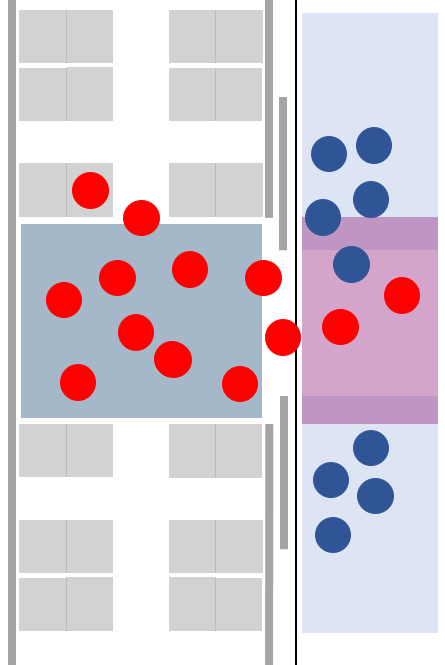
\includegraphics[angle=270, width=0.5\textwidth]{pictures/model/kognitive_heuristic_model/boarding_sketch.png}
	\caption{Skizze zur Darstellung der Zwischenzielbereiche und Zielbereiche von Einsteigen aus der Vogelperspektive: Die Zwischenzielbereiche sind in hellblau und lila, der Zielbereich in dunkelblau eingezeichnet.}
	\label{fig:SkizzeEinsteiger}
\end{figure} 
Der Zwischenzielbereich der Einsteiger, ist in dieser Abbildung, \figurename \ref{fig:SkizzeEinsteiger} in hellblau eingezeichnet. Zu diesem Zwischenziel kann auch der in lila dargestellte Bereich, der "`Im Weg"'-Bereich werden, wenn eine Person aufgrund der Heuristik im Weg steht. Der Zielbereich der Einsteiger ist in dunkelblau dargestellt.

Platzmacher starten im Wagon und gehen zunächst auch in die Wartebereiche neben den Türen, danach ist ihr Ziel dasselbe wie bei den Einsteigern, siehe \figurename \ref{fig:SkizzePlatzmacher}.
\begin{figure}[H]
	\centering
		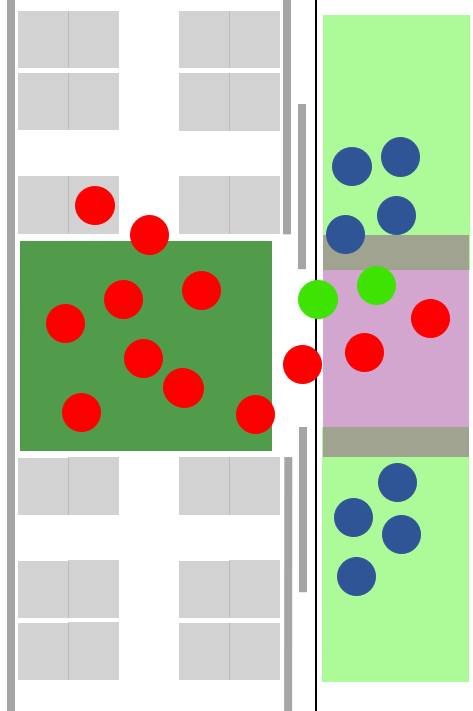
\includegraphics[angle=270, width=0.5\textwidth]{pictures/model/kognitive_heuristic_model/spacemaker_sketch.png}
	\caption{Skizze zur Darstellung der Zwischenzielbereiche und Zielbereiche von Platzmachern aus der Vogelperspektive: Platzmacher werden durch grüne Kreise dargestellt. Zwischenzielbereiche sind in hellgrün und lila, der Zielbereich in dunkelgrün eingezeichnet.}
	\label{fig:SkizzePlatzmacher}
\end{figure}
Der Zwischenzielbereich der Platzmacher, ist in hellgrün eingezeichnet. Zu diesem Zwischenziel kann auch, der in lila dargestellte Bereich, der "`Im Weg"'-Bereich werden, wenn eine Person aufgrund der Heuristik im Weg steht. Der Zielbereich der Platzmacher ist in dunkelgrün dargestellt.
\subsection{Grenzen des Modells}
In meinem Fahrgastwechsel-Modell, wird immer nur eine Tür des Zuges modelliert. Wie sich Personen für eine Tür oder einen Wagon entscheiden, wird somit außer Acht gelassen. Auch ein Umentscheiden einer Person an einer anderen Tür auszusteigen als zunächst geplant wird in diesem Modell nicht bearbeitet, ein Verhalten das auf ein paar der Videos aufgenommen wurde.\\
In meinem Modell weichen Personen, die "`im Weg stehen"' nicht aus, wenn sich andere Personen auf sie zubewegen oder sich an ihnen vorbei drängen. Dieses Verhalten wurde auf Videos von Personen gezeigt, die den Weg anderer versperren. Dieses Verhalten wird jedoch nicht in das Modell mit aufgenommen. \\
In meinem Modell steigen alle im Zug vorhandenen Personen aus dem Zug aus, um auf den Bahnsteig zu gelangen oder Platz zu machen. Personen, die im Zug bleiben und möglicherweise einen Einfluss auf die Fahrgastwechselzeit besitzen, werden nicht modelliert. Zudem gibt es in meinem Modell keine Personen am Bahnsteig, die nicht an der Tür einsteigen wollen. \\
Eine weitere Grenze meines Modells betrifft die Platzmacher. Platzmacher reagieren auf das Bedürfnis von Personen hinter ihnen im Wagon. Sie treten auf, wenn Aussteiger hinter ihnen aus dem Wagon drängen und der Platzmacher keine Möglichkeit hat diesen innerhalb des Wagons auszuweichen. In meinem Modell werden Platzmacher jedoch einfach zu einer übergebenen Anzahl eingesetzt, da kein Zusammenhang zwischen der Anzahl der Aussteiger und dem Auftreten von Platzmachern hergestellt werden konnte und eine Information über die Anzahl der Personen im Wagon nicht erhoben wurde.
\subsection{Umsetzung der Auswertungen}
Bevor ich die Algorithmen für den Fahrgastwechsel und die darin enthaltenen Algorithmen für die Heuristiken erkläre, beschreibe ich in den nächsten Abschnitten, wie die Auswertungen im Modell dargestellt werden sollen.
\subsubsection{Fahrgastwechselzeit}
Die Auswertungen der Fahrgastwechselzeit \ref{Zeiten} werden nicht direkt im Modell verwendet. Sie dienen nur der Validierung und Kalibrierung des Modells. Mit dem Vergleich der aufgenommenen Wechselzeiten mit den Wechselzeiten einer Simulation könnten die Parameter des Algorithmus angepasst werden. Zudem kann mit ihnen nach Simulationen mit diesem Modell überprüft werden ob diese reale Ergebnisse liefern, und das Modell somit Valide ist.
\subsubsection{Gruppen}
Wie im Abschnitt \ref{Gruppen} bereits erklärt, kann die Auswertung für Gruppen nicht direkt in die Software von crowd:it eingesetzt werden. Hier muss zunächst die Übergabe der Gruppen verändert werden. Deshalb werden Gruppen in diesem Modell nicht umgesetzt.
\subsubsection{Verhaltensweisen und Merkmale}
In der Auswertung der Verhaltensweisen und Merkmale, Abschnitt \ref{Verhalten}, kam ich zu dem Schluss, dass das Merkmal "`sperrig"' sowie die Verhaltensweisen "`früher Einsteigen"' und "`im Weg Stehen"' im Modell dargestellt werden sollen. 

Um das Merkmal "`sperrig"' umzusetzen, soll die Schulterbreite der Personen, die in crowd:it angegeben werden kann, verwendet werden. Aus den Daten ergibt sich für den Mittelwert des Anteils von Sperrigen Personen pro Tür ein Anteil von 4.05 \%. Damit ich dieses Merkmal umsetzten kann wird bei 4 \% der Population des Fahrgastwechsel die Schulterbreite auf das 1.5 Fache der ursprünglichen Schulterbreite erhöht. Durch diese Erhöhung werden Personen sperrig und es ist nicht mehr immer möglich zu zweit durch die Tür zu gehen.

Die Verhaltensweisen "`früher Einsteigen"' und "`im Weg Stehen"' setze ich mit den Heuristiken der Prozesstypen um. Bei den Heuristiken der normalen und aggressiven Einsteiger wird abgefragt, wie viel Platz in der Tür vorhanden ist. Ab einer bestimmten Breite Platz in der Tür (genauer erklärt in \ref{EM}), beginnen diese Einsteiger mit dem Einsteigen. So steigen Normale und Aggressive früher ein, wenn Platz in der Tür ist, auch wenn Personen noch aussteigen. Da für Platzmacher die "`Einsteigeprozess"'-Heuristik verwendet wird, tritt durch mein Modell auch bei diesem Prozesstypen das Verhalten "`früher Einsteigen"' auf.\\
Die Verhaltensweise "`im Weg Stehen"' wird in meinem Modell von aggressiven Einsteigern und Platzmachern gezeigt. Hier wird die Verhaltensweise für Platzmacher umgesetzt, indem sie die "`Einsteigeprozess"'-Heuristik verwenden, wenn sie aus dem Wagon ausgestiegen sind. Durch die "`aggressive Platzsuche"'-Heuristik wird die Verhaltensweise "`Im Weg Stehen"' umgesetzt, die in \ref{Verhalten} als signifikant für den Prozess eingestuft wurde. Es wird dazu angenommen, dass diese Verhaltensweise nur auftritt, wenn aggressive Personen vorne oder neben der vordersten Person im Wartebereich keinen Platz finden.

Eine weitere Verhaltensweise die ich in \ref{Verhalten} untersucht habe, ist das Platz machen. Dieses Verhalten wird durch die Modellierung der Prozesstypen Platzmacher umgesetzt. Bei der Auswertung kam ich zu Ergebnis, dass das Vorkommen von Platzmachern nicht durch die Anzahl der Aussteiger abgeschätzt werden kann. Deshalb wird die Anzahl der Platzmacher manuell übergeben, dabei können die, in \ref{Beschreibung der Daten} angegebenen Anteile als Referenz verwendet werden.
\subsubsection{Typen von Personen}
In der Auswertung \ref{Typen} kam ich zu dem Fazit, dass die unterschiedlichen Typen aggressiv, defensiv und normal dargestellt werden sollen, da sie einen signifikanten Anteil besitzen. Im Modell modelliere ich also die in \ref{Tabelle der Typen} angegebenen Verhaltensweisen durch die, die unterschiedlichen Typen auf den von mir erstellten Videos erkannt wurden. Die Verhaltensweise für normale Personen, durch die Tür gehen, wenn genügend Platz in der Tür ist, wurde durch die "`Einsteigeprozess"'-Heuristik umgesetzt. Hierbei wird der Platz in der Tür berechnet, ist dieser größer oder gleich dem 1.2 Fachen der normalen Person, so beginnt diese mit dem Einsteigen. Für Aussteiger wurde dies durch die ebenfalls ausgewerteten Startzeiten umgesetzt. Bei Aussteigern ist der Platz in der Tür dadurch bestimmt, wie weit die Tür geöffnet ist. Nachdem es schwierig ist, in einer Simulation darzustellen, wie weit eine Tür geöffnet ist wurden für Aussteiger die Startzeiten verwendet. Hierbei wird aus dem Intervall der Startzeiten für normale Aussteiger zufällig eine Startzeit für die Person ausgewählt. Es wird dabei angenommen, dass die Startzeiten normal verteilt sind. Auch für aggressive Personen wurde das Merkmal, dass sie durch die Tür gehen, wenn etwas Platz in der Tür ist, durch die Abfrage des Platzes in der Tür und der zufälligen Wahl einer Startzeit aus dem Intervall für aggressive umgesetzt. Das Merkmal für defensive, die nur durch die Tür gehen, wenn keine andere Person in der Tür ist, wird umgesetzt, indem die Heuristik von Michael Seitz angepasst wird. Im Modell von Michael Seitz gehen Personen einen Schritt nicht, wenn dieser zu einer Kollision führt. In meinem Modell nehmen defensive Personen den Schritt auch dann nicht, wenn sie durch diesen den Türbereich betreten würden und sich in diesem gerade eine Person befindet. Sind sie bereits im Türbereich gehen sie jedoch normal durch die Tür. Das sie normal durch die Tür gehen, sobald sie den Türbereich betreten haben, verhindert, dass eine Person stehen bleibt, wenn eine Person nach ihr den Türbereich betritt. Ein weiteres Merkmal von aggressiven Typen ist, dass sie sich vor andere Personen drängen und ihnen dabei sogar in den Weg laufen. Deshalb wird für diese Typen die "`Follower"'-Heuristik angepasst. In der "`Follower"'-Heuristik, die von normalen und defensiven verwendet wird, sucht die Person zunächst eine Person der sie folgen kann, wenn auf dem Weg zum Ziel ein Hindernis liegt. Erst wenn kein Leader gefunden wird, versuchen diese Personen, ihre nächste Position durch die "`Sideways evasion"'-Heuristik zu finden. Aggressive Typen verwenden in meinem Modell jedoch zunächst die "`Sideways evasion"'-Heuristik. Wird hierdurch keine neue mögliche Position gefunden, versuchen auch aggressive Typen einer Person zu folgen, um voran zu kommen. Dadurch überholen sie Personen vor sich. Um darzustellen, dass Aggressive auch in den Weg laufen, gehen diese im Algorithmus immer zuerst ihren Schritt, daraufhin versuchen Normale und dann Defensive sich voran zubewegen. Durch die "`Platzsuche"'-Heuristik wird dargestellt, dass normale Platzmacher sich so weit vorne wie möglich in den Wartebereich stellen, Defensive sich hinter die letzte Person im Wartebereich stellten und Aggressive immer vor die erste Person stellen. Die Heuristik wird in der Heuristik des Einsteigeprozesses verwendet, welcher wiederum von Platzmachern nach dem Aussteigen verwenden wird. Bei diesen Heuristiken suchen Normale nach dem nächsten freien Platz nahe an der Tür und defensive stellen sich hinter die letzte Person im Wartebereich. Aggressive hingegen wollen sich immer ganz vorne in den Wartebereich stellen. Ist vor oder neben der ersten Person kein Platz, so Positionieren sie sich im "`Im Weg"'-Bereich. Auch die ausgewerteten Startzeiten werden im Modell verwendet, wie für Normale und Aggressive bereits erwähnt. Auch für Defensive wird die Startzeit zufällig, diesmal aus dem Intervall der Startzeiten für Defensive, gewählt.
\section{Algorithmus} \label{Algorithmus}
Zur Erklärung der Heuristiken wird zunächst das Prozessdiagramm beschrieben und daraufhin ein Pseudocode angegeben, mit dem dieses umgesetzt werden kann. Dabei wird immer ein Schritt des Agenten dargestellt. In der Simulation werden die Heuristiken also so oft wiederholt, bis die Person den Zielbereich erreicht hat. Zunächst wird der Einsteigeprozess, anschließend der Ausstiegsprozess und zum Schluss der Platzmachprozess erläutert. Bei der Erklärung der "`Einsteigeprozess"'-Heuristik, werden zudem die Algorithmen der kognitiven Heuristiken nach \cite{Seitz.2016} beschrieben.
\subsection{Einsteiger-Heuristik} \label{EM}
Das Prozessdiagramm für die Heuristik des Einsteigeprozess, ist in \figurename \ref{fig:EH} dargestellt. 
\begin{figure}[H]
	\centering
		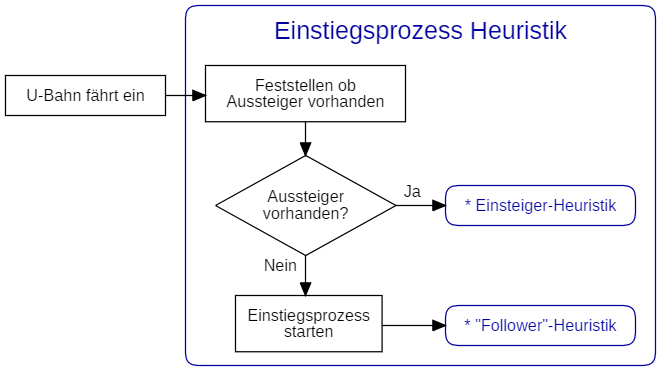
\includegraphics[width=0.9\textwidth]{pictures/model/algorithm/boarding/boarding_process.png}
	\caption{Prozessdiagramm der Einsteiger: "`Einsteigeprozess"'-Heuristik.}
	\label{fig:EH}
\end{figure}
Will eine Person an einer Tür einsteigen, so wird zunächst überprüft ob an dieser Tür Aussteiger vorhanden sind. Ist dies nicht der Fall, so können die Einsteiger durch Verwendung der "`Follower"'-Heuristik, bei aggressiven Einsteigern durch der "`aggressive Follower"'-Heuristik, sofort mit dem Einsteigen in den Zug beginnen. Gibt es jedoch Personen, die durch diese Tür auf den Bahnsteig gelangen wollen, so wird für die unterschiedlichen Typen die jeweilige "`Einsteiger"'-Heuristik verwendet. Der Algorithmus des Einsteigeprozesses, könnte im Code wie folgt umgesetzt werden:

\begin{algorithm} [H]
	\caption{"`Einsteigeprozess"'-Heuristik}
	\SetKwInOut{Output}{Output}
	\SetKwProg{BoardingHeuristic}{BoardingHeuristic}{}{}
	
	\Output{$pos_p$ nächste gewünschte (eng.: "`preferred"') Position}
	\BoardingHeuristic{} {
		Überprüfen ob Aussteiger vorhanden \\
		Typ der Person ist $T$\\
		\If{Aussteiger vorhanden} {
			\uIf{$T$ ist defensiv} { 
				$pos_p = $ \textbf{DefensiveBoardingHeuristic}
			}\uElseIf {$T$ ist normal} {
				$pos_p = $ \textbf{NormalBoardingHeuristic} 	
			} \Else {
				$pos_p = $ \textbf{AggressiveBoardingHeuristic}
			}
		} \Else {
			Ziel des Agenten auf den Bereich im Inneren des Wagons setzten \\
			\If{$T$ ist aggressiv} {
				$pos_p = $ \textbf{AggressiveFollowerHeuristic}		
			} \Else {
				$pos_p = $ \textbf{FollowerHeuristic}		
			}
		}
		\Return $pos_p$
	}
\end{algorithm}

Gibt es keine Aussteiger, so muss die "`Einsteige"'-Heuristik für den entsprechenden Typ nicht verwendet werden, da diese auf dem Vorkommen von Aussteigern beruhen. Die Einsteiger können sofort mit der entsprechenden "`Follower"'-Heuristik mit dem Einsteigen beginnen. Dazu wird das Ziel des Agenten auf den Bereich im Inneren des Zuges gesetzt. Das Ziel des Agenten wird bei Einsteigern erst im Algorithmus festgelegt, da sich das Ziel im Laufe des Algorithmus auf ein Ziel im Wartebereich ändern kann, wenn die Person nicht direkt einsteigen kann. Dieser Fall wird in den unterschiedlichen "`Einsteige"'-Heuristiken abgeprüft. Bevor die Heuristiken für normale, defensive und aggressive Einsteiger beschrieben werden, wird zunächst der Algorithmus der "`Follower"'-Heuristik beschrieben. Dieser Algorithmus, wird auch im Ausstiegs- und Platzmachprozess verwendet.

\cite{Seitz.2016} definiert die "`Follower"'-Heuristik, wie in \figurename \ref{fig:followerHeuristik} dargestellt.
\begin{figure}[H]
	\centering
		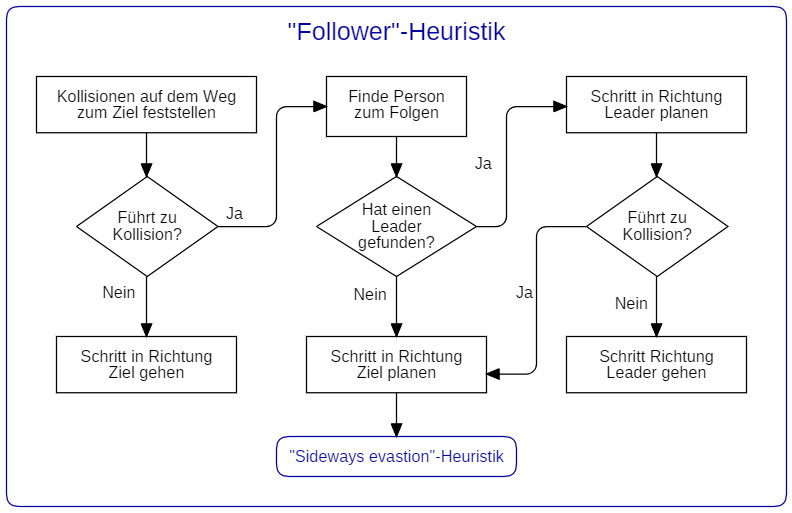
\includegraphics[width=1.0\textwidth]{pictures/model/algorithm/heuristics/follower_heuristic.png}
	\caption{Prozessdiagramm der "`Follower"'-Heuristik nach \cite{Seitz.2016}.}
	\label{fig:followerHeuristik}
\end{figure}
Wird bei der "`Follower"'-Heuristik eine Kollision auf dem Weg zum Ziel erkannt, so versucht der Agent die nächste Person zu finden, die in dieselbe Richtung geht. Ist ein solcher Leader gefunden, geht der Agent seinen nächsten Schritt in Richtung dieses Leaders. Wenn kein Leader gefunden wird oder der Schritt in Richtung Leader zu einer Kollision führen würde, so wird die "`Sideways evasion"'-Heuristik verwendet (\cite{Seitz.2016}). Der Pseudocode der "`Follower"'-Heuristik mit angepasster Abfrage für defensive kann in Algorithmus \ref{alg:Follower} betrachtet werden.
\clearpage
\begin{algorithm} [H]
	\caption{"`Follower"'-Heuristik}
	\label{alg:Follower}
	\SetKwInOut{Output}{Output}
	\SetKwProg{FollowerHeuristic}{FollowerHeuristic}{}{}
	
	\Output{$pos_p$ nächste gewünschte (eng.: "`preferred"') Position}
	\FollowerHeuristic{} {
		Zielrichtung bestimmen \\
		Direkter Pfad zum Ziel berechnen \\
		Pfad auf Kollisionen prüfen \\
		$T_d$ ist \True wenn Typ der Person $T$ defensiv ist, \False falls nicht \\
		\If{Weg führt zu Kollision} {
			Finde Person $L$ zum folgen \\
			\If{$L$ gefunden} { 
				Schritt $pos_L$ in Richtung Leader $L$ berechnen \\
				\If{$pos_L$ führt zu Kollision \Or ($T_d$ \Andnot \textbf{StepPossible}$(pos_{current}, pos_{L})$)} {
					$pos_p$ = \textbf{SidewaysEvasionHeuristic}
				} \Else {
					Schritt in Richtung Leader gehen: $pos_p = pos_L$ 
				}
			} \Else {
				$pos_p$ = \textbf{SidewaysEvasionHeuristic}	
			}
		} \Else {
			nächste Position $pos_{Ziel}$ in Richtung Ziel berechnen \\
			Schritt in Richtung Ziel gehen: $pos_p = pos_{Ziel}$		
		}
		\Return $pos_p$
	}
\end{algorithm}

Liegt auf dem Weg ein Hindernis, wird versucht eine Person der gefolgt werden kann, ein Leader, zu finden. Wird kein Leader gefunden, wird der Algorithmus \ref{alg:SidewaysEvasion} der "`Sideways Evasion"'-Heuristik verwendet, um den nächsten Schritt zu finden. Für die Abfrage bei defensiven Typen wird dabei der Algorithmus \ref{alg:StepPossible} verwendet, um zu überprüfen ob die defensive Person einen Schritt gehen kann. 
\clearpage
\begin{algorithm} [H]
	\caption{Test für defensive Agenten}
	\label{alg:StepPossible}
 	\SetKwInOut{Input}{Input}
 	\SetKwInOut{Output}{Output}
	\SetKwProg{StepPossible}{StepPossible}{}{}
	
	\Input{$pos_{current}$ aktuelle Position des Agenten \newline
	$pos_{next}$ nächste gewünschte Position des Agenten}
	\Output{Boolean Wert, der angibt ob die nächste Position für defensive Agenten möglich ist: \True, wenn möglich }
	\StepPossible{$(pos_{current}$, $pos_{next})$} {
		\If{$pos_{current} \notin$ Türbereich \AND $pos_{next} \in$ Türbereich \AND andere Person im Türbereich} {
		\Return \False
		}\Else {
		\Return \True
		}
	}
\end{algorithm} 

Um herauszufinden ob der nächste Schritt für die Person möglich ist, wird überprüft, ob die Person sich derzeit außerhalb des Türbereich befindet, mit dem nächsten Schritt in den Türbereich eintreten würde und ob sich im Moment eine andere Person im Türbereich befindet. Sind diese Bedingungen gegeben, gibt die Funktion den Boolean Wert "`False"' zurück, da ein Schritt in diesem Fall, in diese Richtung nicht möglich ist. Für die Überprüfung wird der Funktion die aktuelle Position und die zu überprüfende Position übergeben.

Neben dem \textbf{StepPossible} Algorithmus wird in der "`Follower"'-Heuristik auch der Algorithmus \ref{alg:SidewaysEvasion} \textbf{SidewaysEvasionHeuristic} verwendet. Die "`Sideways evasion"'-Heuristik wird in \figurename \ref{fig:sidewayHeuristik} erläutert.
\begin{figure}[H]
	\centering
		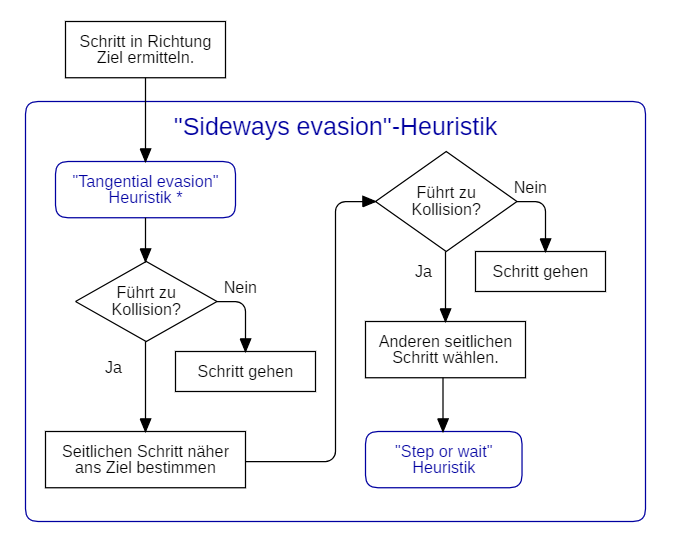
\includegraphics[width=0.9\textwidth]{pictures/model/algorithm/heuristics/sideways_evasion_heuristic.png}
	\caption{Prozessdiagramm der "`Sideways Evasion"'-Heuristik nach \cite{Seitz.2016}.}
	\label{fig:sidewayHeuristik}
\end{figure} 
Bei der "`Sideways evasion"'-Heuristik versuchen die Agenten zunächst die "`Tangential evasion"'-Heuristik zu verwenden, um zum Ziel zu gelangen. Dabei ist zu beachtet, dass die "`Step or wait"'-Heuristik die in  der "`Tangential evasion"'-Heuristik verwendet wird hier nicht angewandt wird. Gelingt das tangentiale Ausweichen nicht, wird versucht seitlich auszuweichen. Die "`Step or wait"'-Heuristik wird von den Agenten erst dann eingesetzt, wenn weder tangentiales noch seitliches Ausweichen möglich ist (\cite{Seitz.2016}). Der Algorithmus für die "`Sideways evasion"'-Heuristik mit meiner Anpassung für defensive Typen ist in Algorithmus \ref{alg:SidewaysEvasion} dargestellt.
\clearpage
\begin{algorithm} [H]
	\caption{"`Sideways evasion"'-Heuristik}
	\label{alg:SidewaysEvasion}
	\SetKwInOut{Output}{Output}
	\SetKwProg{SidewaysEvasionHeuristic}{SidewaysEvasionHeuristic}{}{}
	
	\Output{$pos_p$ nächste gewünschte (eng.: "`preferred"') Position}
	\SidewaysEvasionHeuristic{} {
		$pos_t =$ \textbf{TangentialEvasionHeurisic} \\
		$T_d$ ist \True wenn Typ der Person $T$ defensiv ist, \False falls nicht \\
		\If{zurückgegebene Position $pos_t$ ist $pos_{current}$} {
			speichern des Bereichs des Hindernisses oder Agenten $K$ \\
			berechnen beider seitlichen Umgehungsschritte $pos_c$ und $pos_d$ in Relation zu $K$ \\
			Position $pos_c$ hat die kleinerer Distanz zum Ziel \\
			\If{$pos_c$ führt zu Kollision \Or ($T_d$ \Andnot \textbf{StepPossible}$(pos_{current}, pos_{c})$} {
				\If{$pos_d$ führt zu Kollision \Or ($T_d$ \Andnot \textbf{StepPossible}$(pos_{current}, pos_{d})$} {
					In aktueller Position verbleiben $pos_p = pos_{current}$
				} \Else {
						zweiten seitlichen Schritt in Richtung Ziel gehen $pos_p = pos_d$
				}
			} \Else {
				ersten seitlichen Schritt in Richtung Ziel gehen $pos_p = pos_c$
			}
		} \Else {
			Schritt aus \textbf{TangentialEvasionHeuristic} gehen $pos_p = pos_{t}$		
		}
		\Return $pos_p$
	}
\end{algorithm}

Im \textbf{SidewaysEvasionHeuristic} Algorithmus wird zunächst der \textbf{TangentialEvasionHeuristic} Algorithmus durchgeführt. Gibt dieser Algorithmus als nächste erwünschte Position die jetzige Position des Agenten zurück, war ein direkter Schritt zum Ziel nicht möglich, und auch die Umgehungsschritte konnten nicht gewählt werden. Ist dies der Fall wird versucht seitlich auszuweichen.
Die "`Tangential evasion"'-Heuristik kann in \ref{fig:tangentialHeuristik} betrachtet werden.
\begin{figure}[H]
	\centering
		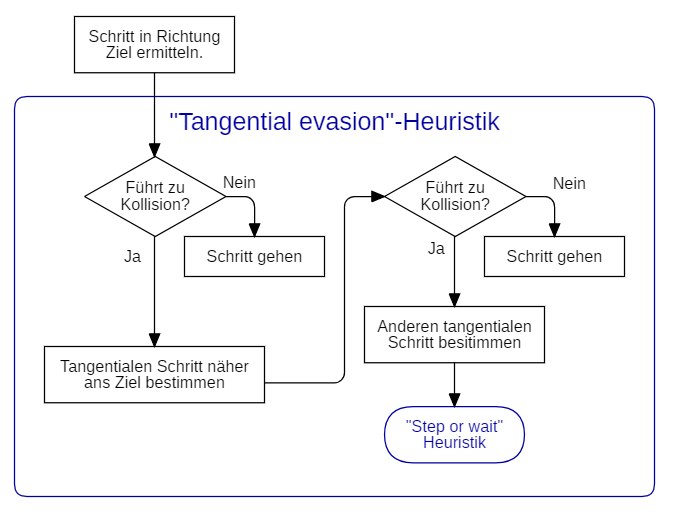
\includegraphics[width=0.9\textwidth]{pictures/model/algorithm/heuristics/tangential_evasion_heuristic.png}
	\caption{Prozessdiagramm der "`Tangential evasion"'-Heuristik nach \cite{Seitz.2016}.}
	\label{fig:tangentialHeuristik}
\end{figure} 
Die "`Tangential evasion"'-Heuristik lässt Agenten versuchen Kollisionen tangential auszuweichen. Wenn das tangentiale Ausweichen nicht möglich ist, so wird die "`Step or wait"'-Heuristik verwendet, was bedeutet, dass der Agent in seiner aktuellen Position verbleibt (\cite{Seitz.2016}). Der zugehörige Algorithmus, wird in Algorithmus \ref{alg:TangentialEvasion}, dargestellt.
\clearpage
\begin{algorithm} [H]
	\caption{"`Tangential evasion"'-Heuristik}
	\label{alg:TangentialEvasion}
	\SetKwInOut{Output}{Output}
	\SetKwProg{TangentialEvasionHeuristic}{TangentialEvasionHeuristic}{}{}
	
	\Output{$pos_p$ nächste gewünschte (eng.: "`preferred"') Position}
	\TangentialEvasionHeuristic{} {
		Zielrichtung bestimmen \\
		nächste Position $pos_{Ziel}$ in Richtung Ziel berechnen \\
		$T_d$ ist \True wenn Typ der Person $T$ defensiv ist, \False falls nicht \\
		\If{$pos_{Ziel}$ führt zu Kollision \Or ($T_d$ \Andnot \textbf{StepPossible}$(pos_{current}, pos_{Ziel})$)} {
			speichern des Bereichs des Hindernisses oder Agenten in $K$ \\
			berechnen der tangentialen Umgehungschritte $pos_a$ und $pos_b$ in Relation zu $K$  \\
			Position $pos_a$ ist die Position mit geringerer Distanz zum Ziel \\
			\If{$pos_a$ führt zu Kollision \Or ($T_d$ \Andnot \textbf{StepPossible}$(pos_{current}, pos_{a})$)} {
				\If{$pos_b$ führt zu Kollision \Or ($T_d$ \Andnot \textbf{StepPossible}$(pos_{current}, pos_{b})$)} {
					In aktueller Position verbleiben $pos_p = pos_{current}$
				} \Else {
					zweiten tangentialen Schritt in Richtung Ziel gehen $pos_p = pos_b$
				}
			} \Else {
				ersten tangentialen Schritt in Richtung Ziel gehen $pos_p = pos_a$			
			}
		} \Else {
			Schritt in Richtung Ziel gehen: $pos_p = pos_{Ziel}$		
		}
		\Return $pos_p$
	}
\end{algorithm}
 
Neben den vorgestellten Heuristiken mit der Anpassung für defensive Agenten, definiere ich zudem noch die "`aggressive Follower"'-Heuristik. Diese soll für aggressive Typen eingesetzt werden, da ich davon ausgehe, dass diese Agenten zunächst versuchen die "`Sideways evasion"'-Heuristik zu verwenden, bevor sie einer Person folgen.

\begin{figure}[H]
	\centering
		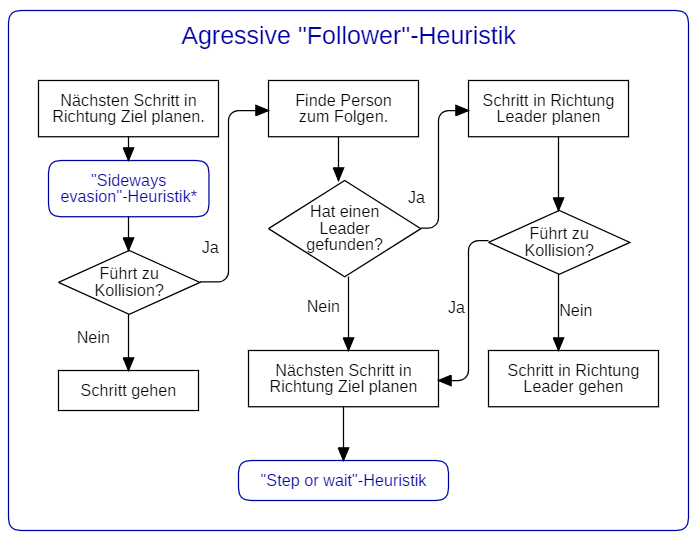
\includegraphics[width=1.0\textwidth]{pictures/model/algorithm/heuristics/aggressive_follower_heuristic.png}
	\caption{Prozessdiagramm der "`aggressiven Follower"'-Heuristik.}
	\label{fig:AFH}
\end{figure}
Bei der "`aggressiven Follower"'-Heuristik versucht der Agent seitlich und tangential auszuweichen, wenn der Weg zum Ziel versperrt ist. Sind auch die Ausweichmöglichkeiten versperrt, so wird versucht der nächsten Person in die gleiche Richtung zu folgen. Wenn jedoch kein Leader gefunden werden kann, oder ein Schritt in die Richtung von diesem zu einer Kollision führen würde, bleibt die Person stehen, sie verwendet die "`Step or wait"'-Heuristik. Der Algorithmus der "`aggressiven Follower"'-Heuristik ist in Algorithmus \ref{alg:aggressiveFollower} eingefügt.
\clearpage
\begin{algorithm} [H]
	\caption{"`aggressive Follower"'-Heuristik}
	\label{alg:aggressiveFollower}
	\SetKwInOut{Output}{Output}
	\SetKwProg{AggressiveFollowerHeuristic}{AggressiveFollowerHeuristic}{}{}
	
	\Output{$pos_p$ nächste gewünschte (eng.: "`preferred"') Position}
	\AggressiveFollowerHeuristic{} {
		$pos_s$ = \textbf{SidewaysEvasionHeuristic}\\
		\If{zurückgegebene Position $pos_s$ ist jetzige Position $pos_{current}$} {
			Finde Person $L$ zum folgen \\
			\If{$L$ gefunden} { 
				Schritt $pos_L$ in Richtung Leader berechnen \\
				\If{$pos_L$ führt zu Kollision} {
					In aktueller Position verbleiben $pos_p = pos_{current}$ 
				} \Else {
					Schritt in Richtung Leader gehen $pos_p = pos_L$
				}
			} \Else {
				In aktueller Position verbleiben $pos_p = pos_{current}$ 	
			}
		} \Else {
			Schritt aus \textbf{SidewaysEvasionHeuristic} gehen: $pos_p = pos_{s}$		
		}
		\Return $pos_p$
	}
\end{algorithm}

Gibt der Algorithmus \textbf{SidewaysEvasionHeuristic} eine neue Position zurück, so wird diese in der \textbf{AggressiveFollwerHeuristic} zurückgegeben. Ist das Ergebnis jedoch die jetzige Position, ein Schritt also nicht möglich, wird versucht einer anderen Person zu folgen.
Nachdem die "`Follower"'-Heuristiken und die Heuristiken die in diesen verwendet werden beschrieben wurden, werden nun die "`Einsteige"'-Heuristiken für Normale, Defensive und Aggressive beschrieben.

\subsubsection{Normaler Einsteiger} 
Für normale Einsteiger wird die "`normaler Einsteiger"'-Heuristik verwendet, welche in \figurename \ref{fig:NEH} gezeigt wird.
\begin{figure}[H]
	\centering
		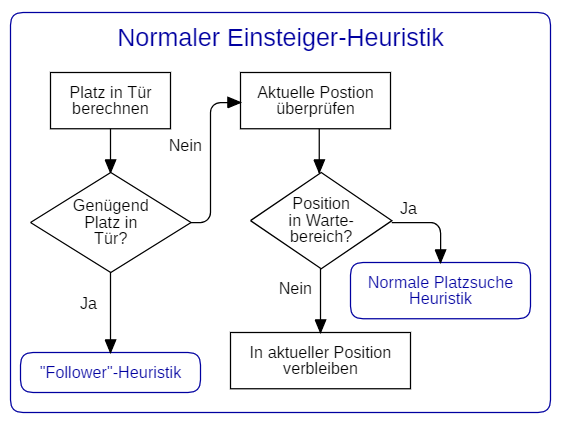
\includegraphics[width=0.8\textwidth]{pictures/model/algorithm/boarding/normal_boarding/normal_boarding_heuristic.png}
	\caption{Prozessdiagramm "`normaler Einsteiger"'-Heuristik.}
	\label{fig:NEH}
\end{figure}
Zunächst wird bei der "`normalen Einsteiger"'-Heuristik berechnet wie viel Platz im Türbereich ist. Ist genügend Platz in der Tür, beschrieben in \ref{Tabelle der Typen}, so beginnt der normale Einsteiger mit dem Einsteigen, was durch die "`Follower"'-Heuristik geschieht. Ist nicht genügend Platz wird überprüft, ob sich der Einsteiger bereits in einem Wartebereich befindet. Ist ein Agent bereits in einem Wartebereich, so verbleibt er in seiner aktuellen Position, er wartet, bis er einsteigen kann. Ist der Agent noch nicht im Wartebereich, so wird die "`normale Platzsuche"'-Heuristik verwendet, die im Anschluss erklärt wird. Zunächst wird jedoch der Algorithmus \ref{alg:NormalBoarding} \textbf{NormalBoardingHeuristic} erklärt. 
\clearpage

\begin{algorithm} [H]
	\caption{"`Normaler Einsteiger"'-Heuristik}
	\label{alg:NormalBoarding}
	\SetKwInOut{Output}{Output}
	\SetKwProg{NormalBoardingHeuristic}{NormalBoardingHeuristic}{}{}
	
	\Output{$pos_p$ nächste gewünschte (eng.: "`preferred"') Position}
	\NormalBoardingHeuristic{} {
		$p=$ Platz in der Tür\\
		\If{$p \geq 1.2 \cdot $ Körperbreite} {
			Ziel des Agenten auf das Innere des Wagons setzen \\
			$pos_p = $ \textbf{FollowerHeuristic} \\
		} \Else {
			\If{aktuelle Position $pos_{current}$ im Wartebereich} {
				In aktueller Position verbleiben $pos_p = pos_{current}$	
			} \Else {
				$pos_p = $ \textbf{normalSpaceFindHeuristic}		
			}
		}
		\Return $pos_p$
	}
\end{algorithm}

Ist in der Tür mehr Platz als das 1.2 Fache der Körperbreite des Agenten, so wird das Ziel des Agenten auf das Innere des Zuges gesetzt, er kann mit der "`Follower"'-Heuristik mit dem Einsteigen beginnen. Ist jedoch nicht genügend Platz in der Tür so wird die "`normale Platzsuche"'-Heuristik verwendet, die eine gewünschte Position für den Einsteiger zurückgibt.
 
Die eben erwähnte "`Platzsuche"'-Heuristik für normale Agenten ist in \figurename \ref{fig:NPH} abgebildet.
\begin{figure}[H]
	\centering
		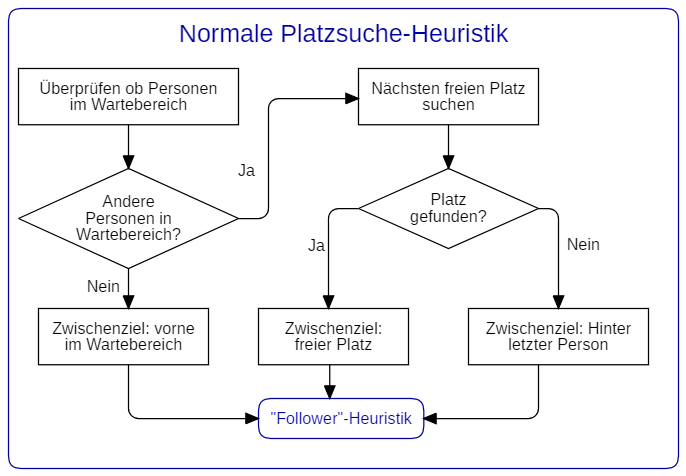
\includegraphics[width=1.0\textwidth]{pictures/model/algorithm/boarding/normal_boarding/normal_space_find_heuristic.png}
	\caption{Prozessdiagramm "`normale Platzsuche"'-Heuristik.}
	\label{fig:NPH}
\end{figure}
Will ein normaler Einsteiger sich an einen Platz im Wartebereich stellen, so wird zunächst überprüft, ob in diesem schon andere Agenten stehen. Steht dort keine Person, so wird das Zwischenziel des Agenten auf den vorderen Bereich der Wartezone gesetzt. Ich nehme an, dass jemand nah an der Tür ist, wenn er nicht weiter von ihr entfernt ist als seine doppelte Schulterbreite. Sind schon Agent im Wartebereich sucht der Agent nach dem nächsten freien Platz in der Nähe der Tür. Kann ein solcher Platz nicht gefunden werden, so wird das Zwischenziel des normalen Einsteigers zur Position hinter der letzten Person. Wurde ein freier Platz gefunden, ist dieser das Zwischenziel des Agenten. Nachdem das Zwischenziel festgelegt wurde bewegt sich der Agent mit Hilfe der "`Follower"'-Heuristik in die Richtung von diesem.
\clearpage
\begin{algorithm} [H]
	\caption{"`Normale Platzsuche"'-Heuristik}
	\SetKwInOut{Output}{Output}
	\SetKwProg{normalSpaceFindHeuristic}{normalSpaceFindHeuristic}{}{}
	
	\Output{$pos_p$ nächste gewünschte (eng.: "`preferred"') Position}
	\normalSpaceFindHeuristic{} {
		\If{andere Person in Wartebereich} {
			Suche nächsten freien Platz $pos_w$ in Wartebereich \\
			\If{Platz gefunden}{
				Ziel des auf $pos_w$ setzen \\
			}\Else{
				Ziel des Agenten auf Platz hinter letzter Person setzen  \\
			}
		} \Else {
			Ziel des Agenten auf Platz vorne im Wartebereich setzten\\
		}
		$pos_p = $ \textbf{FollowerHeuristic} \\
		\Return $pos_p$
	}
\end{algorithm}

Wie im Prozessdiagramm erklärt, wird bei der "`Platzsuche"'-Heuristik für den Einsteiger ein Zwischenziel im Wartereich gewählt. Algorithmisch wird dies Umgesetzt, indem das Ziel des Agenten auf den entsprechenden Platz gesetzt wird. Ist die Person an ihrem Zwischenziel angekommen, genügend Platz in der Tür oder alle Aussteiger ausgestiegen, so wird das Ziel des Agenten durch die vorgestellten Algorithmen für normale Einsteiger wieder auf das Innere des Zuges gesetzt. Bei den "`Platzsuche"'-Heuristiken wird in jedem Simulationsschritt erneut überprüft an welchen Platz sich die Person stellen soll. So wird verhindert, dass sich die Person auf einen Platz stellen will, an dem ein anderer Agent vor ihm ankommt.
\subsubsection{Defensiver Einsteiger}
Das Prozessdiagramm der defensiver "`Einsteiger"'-Heuristik wird in \ref{fig:DEH} gezeigt.
\begin{figure}[H]
	\centering
		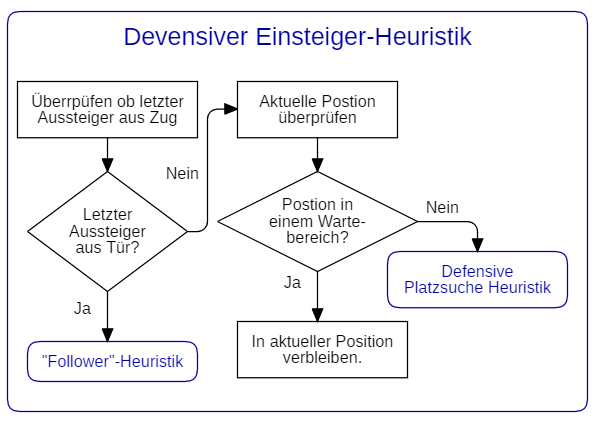
\includegraphics[width=0.9\textwidth]{pictures/model/algorithm/boarding/defensive_boarding/defensive_boarding_heuristic.png}
	\caption{Prozessdiagramm "`defensiver Einsteiger"'-Heuristik.}
	\label{fig:DEH}
\end{figure}
Wie in \figurename \ref{fig:DEH} zu sehen ist, überprüft ein defensiver Einsteiger zunächst, ob der letzte Aussteiger schon ausgestiegen ist.  Ist der letzte Aussteiger aus der Tür, beginnt der defensive Einsteiger mit der "`Follower"'-Heuristik mit dem Einsteigen. Sind noch Aussteiger im Zug, überprüft der Agent seine aktuelle Position. Liegt diese im Wartebereich, verweilte er in seiner aktuellen Position. Ist der Einsteiger noch nicht im Wartebereich, sucht er mit Hilfe der "`defensiven Platzsuche"'-Heuristik einen Platz in diesem. Diese Heuristik kann in \figurename \ref{fig:DPH} betrachtet werden. Im Gegensatz zu normalen Einsteigern, wartet der defensive Einsteiger solange im Wartebereich, bis der letzte Aussteiger den Wagon verlässt, auch wenn genügend Platz ist. 
\clearpage
\begin{algorithm} [H]
	\caption{"`Defensive Einsteiger"'-Heuristik}
	\SetKwInOut{Output}{Output}
	\SetKwProg{DefensiveBoardingHeuristic}{DefensiveBoardingHeuristic}{}{}
	
	\Output{$pos_p$ nächste gewünschte (eng.: "`preferred"') Position}
	\DefensiveBoardingHeuristic{}{
		\If{letzter Aussteiger aus Tür} {
			Ziel auf das Innere des Wagons setzen \\
			$pos_p = $ \textbf{FollowerHeuristic} \\
		} \Else {
			\If{$pos_{current}$ im Wartebereich} {
				In aktueller Position verbleiben $pos_p = pos_{current}$\\
			} \Else {
				$pos_p = $ \textbf{DefensiveSpaceFindHeuristic}	 \\	
			}
		}
		\Return $pos_p$
	}
\end{algorithm}

Bei defensiven Typen wird das Ziel erst auf das Innere des Zuges gesetzt, wenn alle Aussteiger den Zug verlassen haben. Ist dies nicht der Fall, so bleiben sie in ihrer aktuellen Position, wenn sie bereits im Wartebereich angekommen sind oder suchen mit der \textbf{DefensiveSpaceFindHeuristic} einen Platz in eben diesem.

\begin{figure}[H]
	\centering
		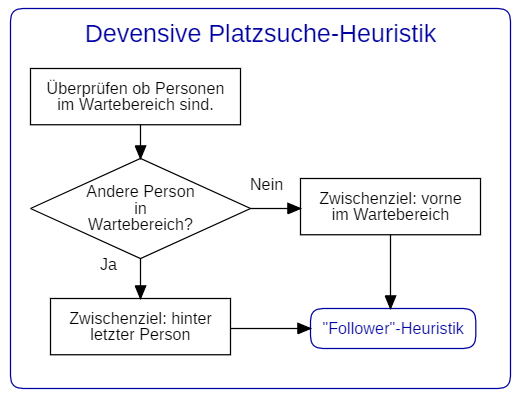
\includegraphics[width=0.8\textwidth]{pictures/model/algorithm/boarding/defensive_boarding/defensive_space_find_heuristic.png}
	\caption{Prozessdiagramm "`defensive Platzsuche"'-Heuristik.}
	\label{fig:DPH}
\end{figure}
In der "`defensiven Platzsuche"'-Heuristik, wählt der Agent als Zwischenziel ebenfalls einen Platz nahe an der Tür, wenn keine andere Person im Wartebereich steht. Ist schon eine Person im Wartebereich, so wählt der defensive Einsteiger immer die Position hinter der letzten wartenden Person im Bereich als sein Zwischenziel. Mit Hilfe der "`Follower"'-Heuristik, bewegt sich der Agent daraufhin zu seinem Zwischenziel. \\
\begin{algorithm} [H]
	\caption{"`Defensive Platzsuche"'-Heuristik}
	\SetKwInOut{Output}{Output}
	\SetKwProg{DefensiveSpaceFindHeuristic}{DefensiveSpaceFindHeuristic}{}{}
	
	\Output{$pos_p$ nächste gewünschte (eng.: "`preferred"') Position}
	\DefensiveSpaceFindHeuristic{} {
		\If{andere Person in Wartebereich} {
			Ziel des Agenten auf Platz hinter letzter Person setzen\\
		} \Else {
			Ziel des Agenten auf Platz vorne im Wartebereich setzen\\
		}
		$pos_p = $ \textbf{FollowerHeuristic} \\
		\Return $pos_p$
	}
\end{algorithm}.

Bei defensiven Agenten gibt es zwei mögliche Zwischenziele im Wartebereich. Entweder ist keine Person im Wartebereich und das Ziel der Agenten wird vom Algorithmus auf einen Platz vorne im Wartebereich gesetzt, oder der Algorithmus wählt einen Platz hinter der letzten Person im Wartebereich.
\subsubsection{Aggressiver Einsteiger}
Die Heuristik der aggressiven Einsteiger in \figurename \ref{fig:AEH} wird in \ref{fig:AEH} erklärt.
\begin{figure}[H]
	\centering
		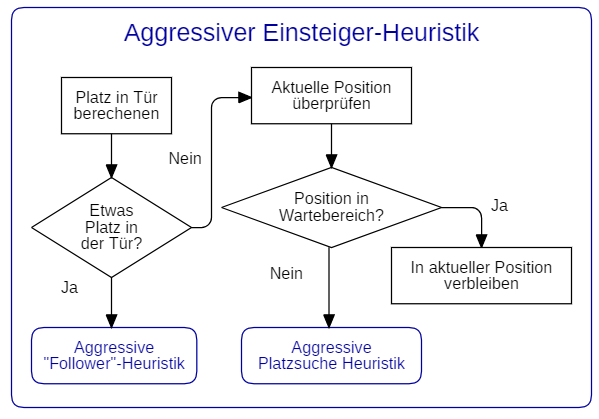
\includegraphics[width=0.8\textwidth]{pictures/model/algorithm/boarding/aggressive_boarding/aggressive_boarding_heuristic.png}
	\caption{Prozessdiagramm "`aggressive Einsteiger"'-Heuristik.}
	\label{fig:AEH}
\end{figure}
Ist etwas Platz (siehe \ref{Tabelle der Typen}) in der Tür, so beginnt der aggressive Einsteiger mit der "`aggressiven Follower"'-Heuristik mit dem Einsteigen. Er hat also eine geringere Schwelle für das Einsteigen als normale oder defensive Einsteiger, die erst bei genügend Platz oder bei Ausstieg des letzten Aussteigers mit dem Einsteigen beginnen. Ist nicht ausreichend Platz in der Tür, so wird die aktuelle Position des Agenten überprüft. Ist dieser noch nicht im Wartebereich, so sucht der aggressive Einsteiger mit der "`aggressiven Platzsuche"'-Heuristik einen Platz in diesem (siehe \figurename \ref{fig:APH}). Ist bereits im Wartebereich so verbleibt er in seiner aktuellen Position.

\begin{algorithm} [H]
	\caption{"`Aggressive Einsteiger"'-Heuristik}
	\SetKwInOut{Output}{Output}
	\SetKwProg{AggressiveBoardingHeuristic}{AggressiveBoardingHeuristic}{}{}
	
	\Output{$pos_p$ nächste gewünschte (eng.: "`preferred"') Position}
	\AggressiveBoardingHeuristic{} {
		$p=$ Platz in der Tür\\
		\If{$p \geq 0.8 \cdot $ Körperbreite} {
			Ziel auf das Innere des Wagons setzen
			$pos_p = $ \textbf{AggressiveFollowerHeuristic}
		} \Else {
			\If{aktuelle Position $pos_current$ im Wartebereich} {
				In aktueller Position verbleiben $pos_p = pos_{current}$	
			} \Else {
				$pos_p = $ \textbf{AggressiveSpaceFindHeuristic}		
			}
		}
		\Return $pos_p$
	}
\end{algorithm}

Im Algorithmus wird als Schwelle für "`etwas Platz"' in der Tür das 0.8 Fache der Körperbreite der Person verwendet. Ist dieser Platz gegeben so wird das Ziel der Person auf das Innere des Wagons gegeben. Sonst sucht der aggressive Einsteiger mit dem Algorithmus \textbf{AggressiveSpaceFindHeuristic} \ref{alg:aggressivSpaceFinder}, nach einem Platz im Wartebereich, wenn er noch nicht in diesem angekommen ist.

\begin{figure}[H]
	\centering
		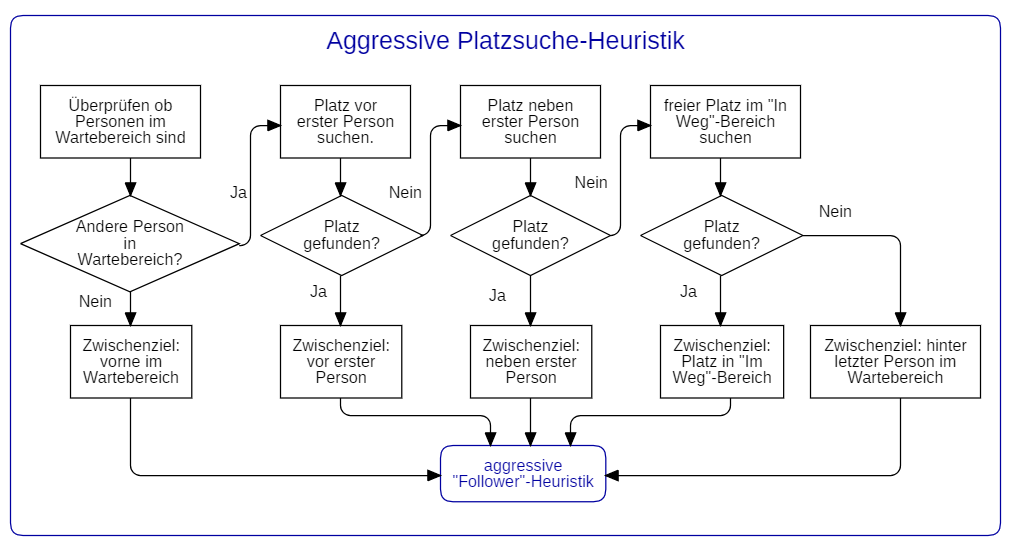
\includegraphics[width=1.0\textwidth]{pictures/model/algorithm/boarding/aggressive_boarding/aggressive_space_find_heuristic.png}
	\caption{Prozessdiagramm "`aggressive Platzsuche"'-Heuristik.}
	\label{fig:APH}
\end{figure}
Ist keine Person im Wartebereich, so wählt der aggressive Agent, genau wie ein defensiver oder normaler, einen Platz nah an der Tür als Zwischenziel. Anders als defensive und normale Typen, will der aggressive Einsteiger jedoch so weit wie möglich vorne stehen, deshalb sucht er nicht nach dem nächsten freien Platz. Stattdessen überprüft der Agent ob vor der ersten Person noch Platz ist, wobei seinem Körper auch leicht in die Tür ragen kann, wenn er sich auf diesen Platz stellt. Es ist also zu vermuten, dass für einen aggressiven Einsteiger auch Platz vor der ersten wartenden Person ist, wenn das 0.8 Fache seiner Körperbreite Platz hat. Ist hier jedoch weniger Platz, so sucht er nach einem Platz neben der ersten Person. Ist hier Platz vorhanden, so wählt er diesen als sein Zwischenziel, auch hier kann sein Körper leicht in die Tür ragen. Ist weder vor noch neben der ersten Person Platz, so sucht ein aggressiver Einsteiger nach einem Platz im "`Im Weg"'-Bereich. Dieser Bereich wurde in der Skizze der Zielbereiche für Einsteiger, \figurename \ref{fig:SkizzeEinsteiger}, bereits dargestellt. Ist hier Platz vorhanden, so wählt er wiederum diesen als Zwischenziel. Ist keiner der genannten Plätze vorhanden, so wählt der Agent als Zwischenziel den Platz hinter der letzten Person im Wartebereich. 
\clearpage
\begin{algorithm} [H]
	\caption{"`Aggressive Platzsuche"'-Heuristik}
	\label{alg:aggressivSpaceFinder}
	\SetKwInOut{Output}{Output}
	\SetKwProg{AggressiveSpaceFindHeuristic}{AggressiveSpaceFindHeuristic}{}{}
	
	\Output{$pos_p$ nächste gewünschte (eng.: "`preferred"') Position}
	\AggressiveSpaceFindHeuristic{} {
		\If{andere Person in Wartebereich} {
			Platz vor erster Person im Wartebereich $pos_{vP}$ suchen \\
			\If{Platz gefunden} {
				Ziel des Agenten auf $pos_{vP}$ setzen \\
			} \Else {
				Platz neben erster Person im Wartebereich $pos_{nP}$ suchen\\
				\If {Platz gefunden} {
				Ziel des Agenten auf $pos_{nP}$ setzen \\		
				} \Else {
					Freien Platz in "`Im Weg"'-Bereich $pos_{iW}$ suchen \\
					\If {Platz gefunden} {
						Ziel des Agenten auf $pos_{iW}$ setzen \\			
					} \Else {
						nächsten freien Platz im Wartebereich $pos_{w}$ suchen \\
						\If {Platz gefunden} {
							$Ziel = pos_w$ \\
						} \Else {
							Ziel des Agenten auf Platz hinter letzter Person im Wartebereich setzen \\					
						}
					}
				}
			} 
		} \Else {
			Ziel des Agenten auf Platz vorne im Wartebereich setzen \\
			
		}
		$pos_p = $ \textbf{AggressiveFollowerHeuristic} \\
		\Return $pos_p$
	}
\end{algorithm}

Bei aggressiven Einsteigern wird das Ziel des Agenten auf einer der möglichen Positionen gesetzt, je nachdem welche frei ist. Mit der "`aggressiven Follower"'-Heuristik bewegt sich die Person dann zu diesem Platz.

\subsection{Aussteiger-Heuristik} \label{AM}
Der Ausstiegsprozess wird mit der "`Ausstiegsprozess"'-Heuristik umgesetzt. Dabei liegt die Unterscheidung der Typen nur in der Wahl der Startzeit der Person, und der Durchführung der "`Follower"'-Heuristik.
\begin{figure}[H]
	\centering
		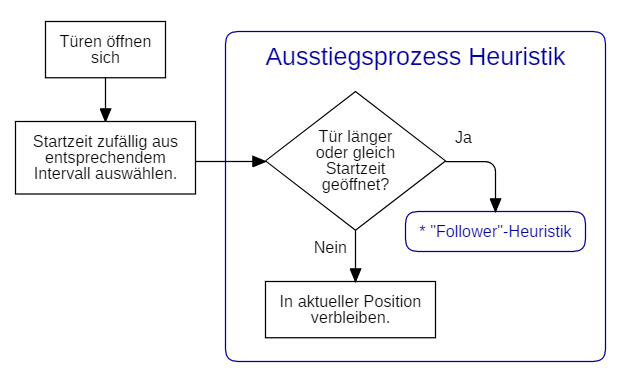
\includegraphics[width=0.8\textwidth]{pictures/model/algorithm/alight/alight_process.png}
	\caption{Prozessdiagramm der Aussteiger: "`Ausstiegsprozess"'-Heuristik.}
	\label{fig:AH}
\end{figure}
Wie in \figurename \ref{fig:AH} zu erkennen, wird die Startzeit des Aussteigers vor dem Ausstiegsprozess festgelegt. Dabei wird diese durch Zufall aus dem entsprechenden Intervall ausgewählt. Die Intervalle wurden hierbei durch die Auswertung in \ref{Startzeiten} ermittelt. Das Startzeitenintervall für defensive liegt zwischen $1.9$ und $2.1$ Sekunden. Für normale liegt es zwischen $1.6$ und $1.8$ Sekunden und für aggressive zwischen $1.3$ und $1.6$ Sekunden. Hierbei nehme ich an, dass die Werte im Intervall normal verteilt sind. Ist die Startzeit gewählt, so beginnt die "`Ausstiegsprozess"'-Heuristik. Dabei verbleibt die Person in ihrer aktuellen Position so lange nicht mehr Zeit seit der Türöffnung vergangen ist, als die Startzeit der Person. Wenn die Tür länger oder gleich der Startzeit geöffnet ist beginnt die Person mit der entsprechenden "`Follower"'-Heuristik den Ausstieg. Dabei wird die "`aggressive Follower"'-Heuristik für aggressive Typen verwendet. 
\clearpage
\begin{algorithm} [H]
	\caption{"`Ausstiegsprozess"'-Heuristik}
	\SetKwInOut{Output}{Output}
	\SetKwProg{AlightHeuristic}{AlightHeuristic}{}{}

	\Output{$pos_p$ nächste gewünschte (eng.: "`preferred"') Position}
	\AlightHeuristic{} {
		Vergangene Sekunden seit Türöffnung in $t$ speichern\\
		Typ der Person ist $T$ \\
		\If{$t <$ Startzeit des Agenten} {
			In aktueller Position verbleiben $pos_{p} = pos_{current}$ 
		} \Else {
			\If{$T$ ist aggressiv} {
				$pos_p = $ \textbf{AggressiveFollowerHeuristic}		
			} \Else {
				$pos_p = $ \textbf{FollowerHeuristic}		
			}
		}
		\Return $pos_p$
	}
\end{algorithm}

Im Algorithmus wird in jedem Schritt überprüft, ob seit der Türöffnung mehr Zeit vergangen ist ist als die Startzeit, ist das der Fall, verbleibt der Agent in seiner aktuellen Position, er wartet, bis die Türen weit genug geöffnet sind. Andernfalls steigt er mit Hilfe der Algorithmen für die "`Follower"'-Heuristik aus.

\subsection{Platzmacher-Heuristik}
Das Platzmacher-Modell wird durch die "`Platzmachprozess"'-Heuristik umgesetzt, die sowohl die "`Ausstiegsprozess"'-Heuristik, als auch die "`Einsteigeprozess"'-Heuristik verwendet.
\begin{figure}[H]
	\centering
		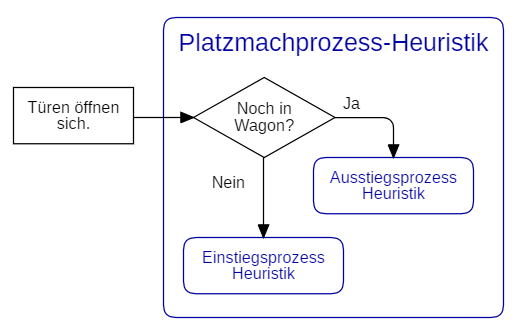
\includegraphics[width=0.7\textwidth]{pictures/model/algorithm/spacemaker/spacemaker_heuristic.png}
	\caption{Prozessdiagramm der Platzmacher: "`Platzmachprozess"'-Heuristik.}
	\label{fig:PH}
\end{figure}
Befindet sich ein Platzmacher im Wagon, so wird die "`Ausstiegsprozess"'-Heuristik (\ref{AM}) verwendet. Will eine Person aussteigen, um Platz zu machen verhält sie sich wie ein Aussteiger. Sobald die Person den Wagon verlassen hat, verhält sie sich jedoch wie ein Einsteiger, sie sucht einen Platz im Wartebereich und steigt daraufhin wieder ein. Dazu wird die "`Einsteigeprozess"'-Heuristik verwendet (\ref{EM}).

\begin{algorithm} [H]
	\caption{"`Platzmachprozess"'-Heuristik}
	\SetKwInOut{Output}{Output}
	\SetKwProg{SpacemakerHeuristic}{SpacemakerHeuristic}{}{}
	
	\Output{$pos_p$ nächste gewünschte (eng.: "`preferred"') Position}
	\SpacemakerHeuristic{} {
		\If{$pos_{current} \in $ Wagon}  {
			$pos_p = $ \textbf{AlightHeuristic}
		} \Else {
			$pos_p = $ \textbf{BoardingHeuristic}	
		}
		\Return $pos_p$
	}
\end{algorithm}

Der Algorithmus des Platzmachprozesses verwendet den Algorithmus \textbf{AlightHeuristic}, wenn sich der Agent noch im Wagon befindet. Ist der Platzmacher aus dem Wagon ausgestiegen, so wird die \textbf{BoardingHeuristic} verwendet.
\section{Modellparameter} \label{Modellparameter}
Das Fahrgastwechsel-Modell beinhaltet die Geometrie des Zuges und Bahnsteigs, sowie die jeweilige Anzahl an Einsteigern, Aussteigern und Platzmachern als Parameter. Zudem wird dem Modell auch die Geometrie der Zielbereiche und Wartereiche, sowie die Geometrie des "`Im Weg"'-Bereiches übergeben. Außerdem werden im Modell die Startzeitenintervalle, sowie der Faktor zur Überprüfung des Platzes in der Tür vorgegeben. Geometrien, für den Zug und die Bereiche, können crowd:it durch CAD Software übergeben werden. Die Parameter für die Anzahl an Einsteigern, Aussteigern und Platzmachern könnte dann in crowd:it als Zahl übergeben werden. 

Da mein Modell nicht in der Software implementiert wurde, ist nicht klar, ob Startzeitenintervalle, Faktoren für die Überprüfung nach Platz in der Tür oder andere "`Floor Field"' Parameter der Software für ein realistisches Modell noch kalibriert werden müssen. Diese Kalibrierung könnte jedoch durch die qualitative Betrachtung einer Simulation, sowie dem Vergleich des Ergebnisses der Simulation mit den ausgewerteten Daten, darunter die Wechselzeiten, stattfinden.